% =============================================================================
% ANEXOS
% =============================================================================

\cleardoublepage
\thispagestyle{empty}
\vspace*{\fill}
\begin{center}
{\Huge\bfseries ANEXOS}
\end{center}
\vspace*{\fill}
\clearpage

\chapter*{ANEXOS}
\addcontentsline{toc}{chapter}{ANEXOS}
\setcounter{section}{0}

% Reiniciar numeración para anexos con letras
\renewcommand{\thesection}{Anexo \Alph{section}}

\section{Guion de entrevista a docentes y psicopedagogos}

A continuación se presenta la estructura de la guía de entrevista semiestructurada utilizada con los cinco docentes de educación básica elemental. La duración promedio de cada entrevista fue de cuarenta minutos y se realizó de manera presencial e individual, previo consentimiento informado por escrito.

\begin{enumerate}[leftmargin=*]
\item ¿Cuántos años de experiencia tiene en la enseñanza de matemáticas en educación básica elemental?
\item ¿Cómo describiría su experiencia general aplicando evaluaciones por competencias en matemáticas?
\item ¿Cuáles son los principales desafíos que enfrenta al diseñar y aplicar evaluaciones a estudiantes de educación básica elemental?
\item ¿Qué herramientas digitales utiliza actualmente, si existen, para apoyar el proceso evaluativo?
\item ¿Qué limitaciones identifica en los métodos tradicionales de evaluación que utiliza?
\item ¿Qué expectativas tendría sobre una aplicación web orientada específicamente a la evaluación por competencias?
\item ¿Qué tipos y formatos de preguntas considera más adecuados para este nivel? (opción múltiple, unir columnas, secuencias, abiertas, etc.)
\item ¿Qué elementos de accesibilidad considera necesarios para estudiantes con diferentes ritmos de aprendizaje?
\item ¿Qué información cree que debe contener un reporte de seguimiento académico para resultar útil al docente?
\item ¿Considera que la retroalimentación motivacional automatizada puede aportar al proceso evaluativo? ¿Por qué?
\end{enumerate}

Las entrevistas con los dos psicopedagogos se desarrollaron bajo un enfoque no estructurado, abordando los siguientes ejes orientadores: (a) barreras cognitivas más frecuentes en la edad de educación básica elemental; (b) recomendaciones específicas de diseño inclusivo; (c) prácticas de retroalimentación que reduzcan la ansiedad evaluativa; y (d) consideraciones para estudiantes con discapacidad intelectual leve.

\section{Cuestionario SUS aplicado en castellano}

Se utilizó la versión validada en español de la \textit{System Usability Scale} (Brooke, 1996), aplicada de forma posterior a la sesión de uso. Los participantes respondieron en una escala Likert de cinco puntos (1 = Totalmente en desacuerdo; 5 = Totalmente de acuerdo).

\begin{enumerate}[leftmargin=*]
\item Creo que me gustaría utilizar este sistema con frecuencia.
\item Encontré el sistema innecesariamente complejo.
\item Pensé que el sistema era fácil de usar.
\item Creo que necesitaría el apoyo de un técnico para poder utilizar este sistema.
\item Las funciones del sistema están bien integradas.
\item Hay demasiada inconsistencia en este sistema.
\item Imagino que la mayoría de las personas aprenderían a utilizar este sistema rápidamente.
\item El sistema me resultó muy difícil de utilizar.
\item Me sentí muy seguro al usar el sistema.
\item Necesité aprender muchas cosas antes de poder utilizar este sistema.
\end{enumerate}

\textbf{Cálculo del puntaje SUS.} Para los ítems impares (1, 3, 5, 7, 9) se resta 1 al valor de la respuesta. Para los ítems pares (2, 4, 6, 8, 10) se resta el valor a 5. La suma de los diez resultados se multiplica por 2,5 para obtener el puntaje final en una escala de 0 a 100.

\section{Cuestionario TAM aplicado en castellano}

Se utilizó una adaptación al español del \textit{Technology Acceptance Model} (Davis, 1989), estructurado en tres dimensiones. Cada ítem se respondió en escala Likert de 1 a 5 (1 = Totalmente en desacuerdo; 5 = Totalmente de acuerdo).

\textbf{Utilidad Percibida (PU).}
\begin{enumerate}[leftmargin=*]
\item Usar Kiddy Quiz me ayuda a evaluar mejor el aprendizaje en matemáticas.
\item Usar Kiddy Quiz hace que mi tarea de evaluación sea más rápida.
\item Usar Kiddy Quiz mejora la calidad de la retroalimentación que recibo/doy.
\end{enumerate}

\textbf{Facilidad de Uso Percibida (PEOU).}
\begin{enumerate}[leftmargin=*,resume]
\item Aprender a usar Kiddy Quiz es fácil para mí.
\item La interacción con la aplicación es clara y comprensible.
\item Encuentro la aplicación flexible al interactuar.
\end{enumerate}

\textbf{Intención de Uso (IU).}
\begin{enumerate}[leftmargin=*,resume]
\item Tengo la intención de seguir usando Kiddy Quiz.
\item Recomendaría Kiddy Quiz a otros compañeros.
\item Si tuviera la oportunidad, usaría Kiddy Quiz frecuentemente.
\end{enumerate}

\section{Diagrama completo de casos de uso del sistema}

\begin{figure}[H]
\centering
\caption{Diagrama completo de casos de uso del sistema Kiddy Quiz.}
\label{fig:anexo_cu}
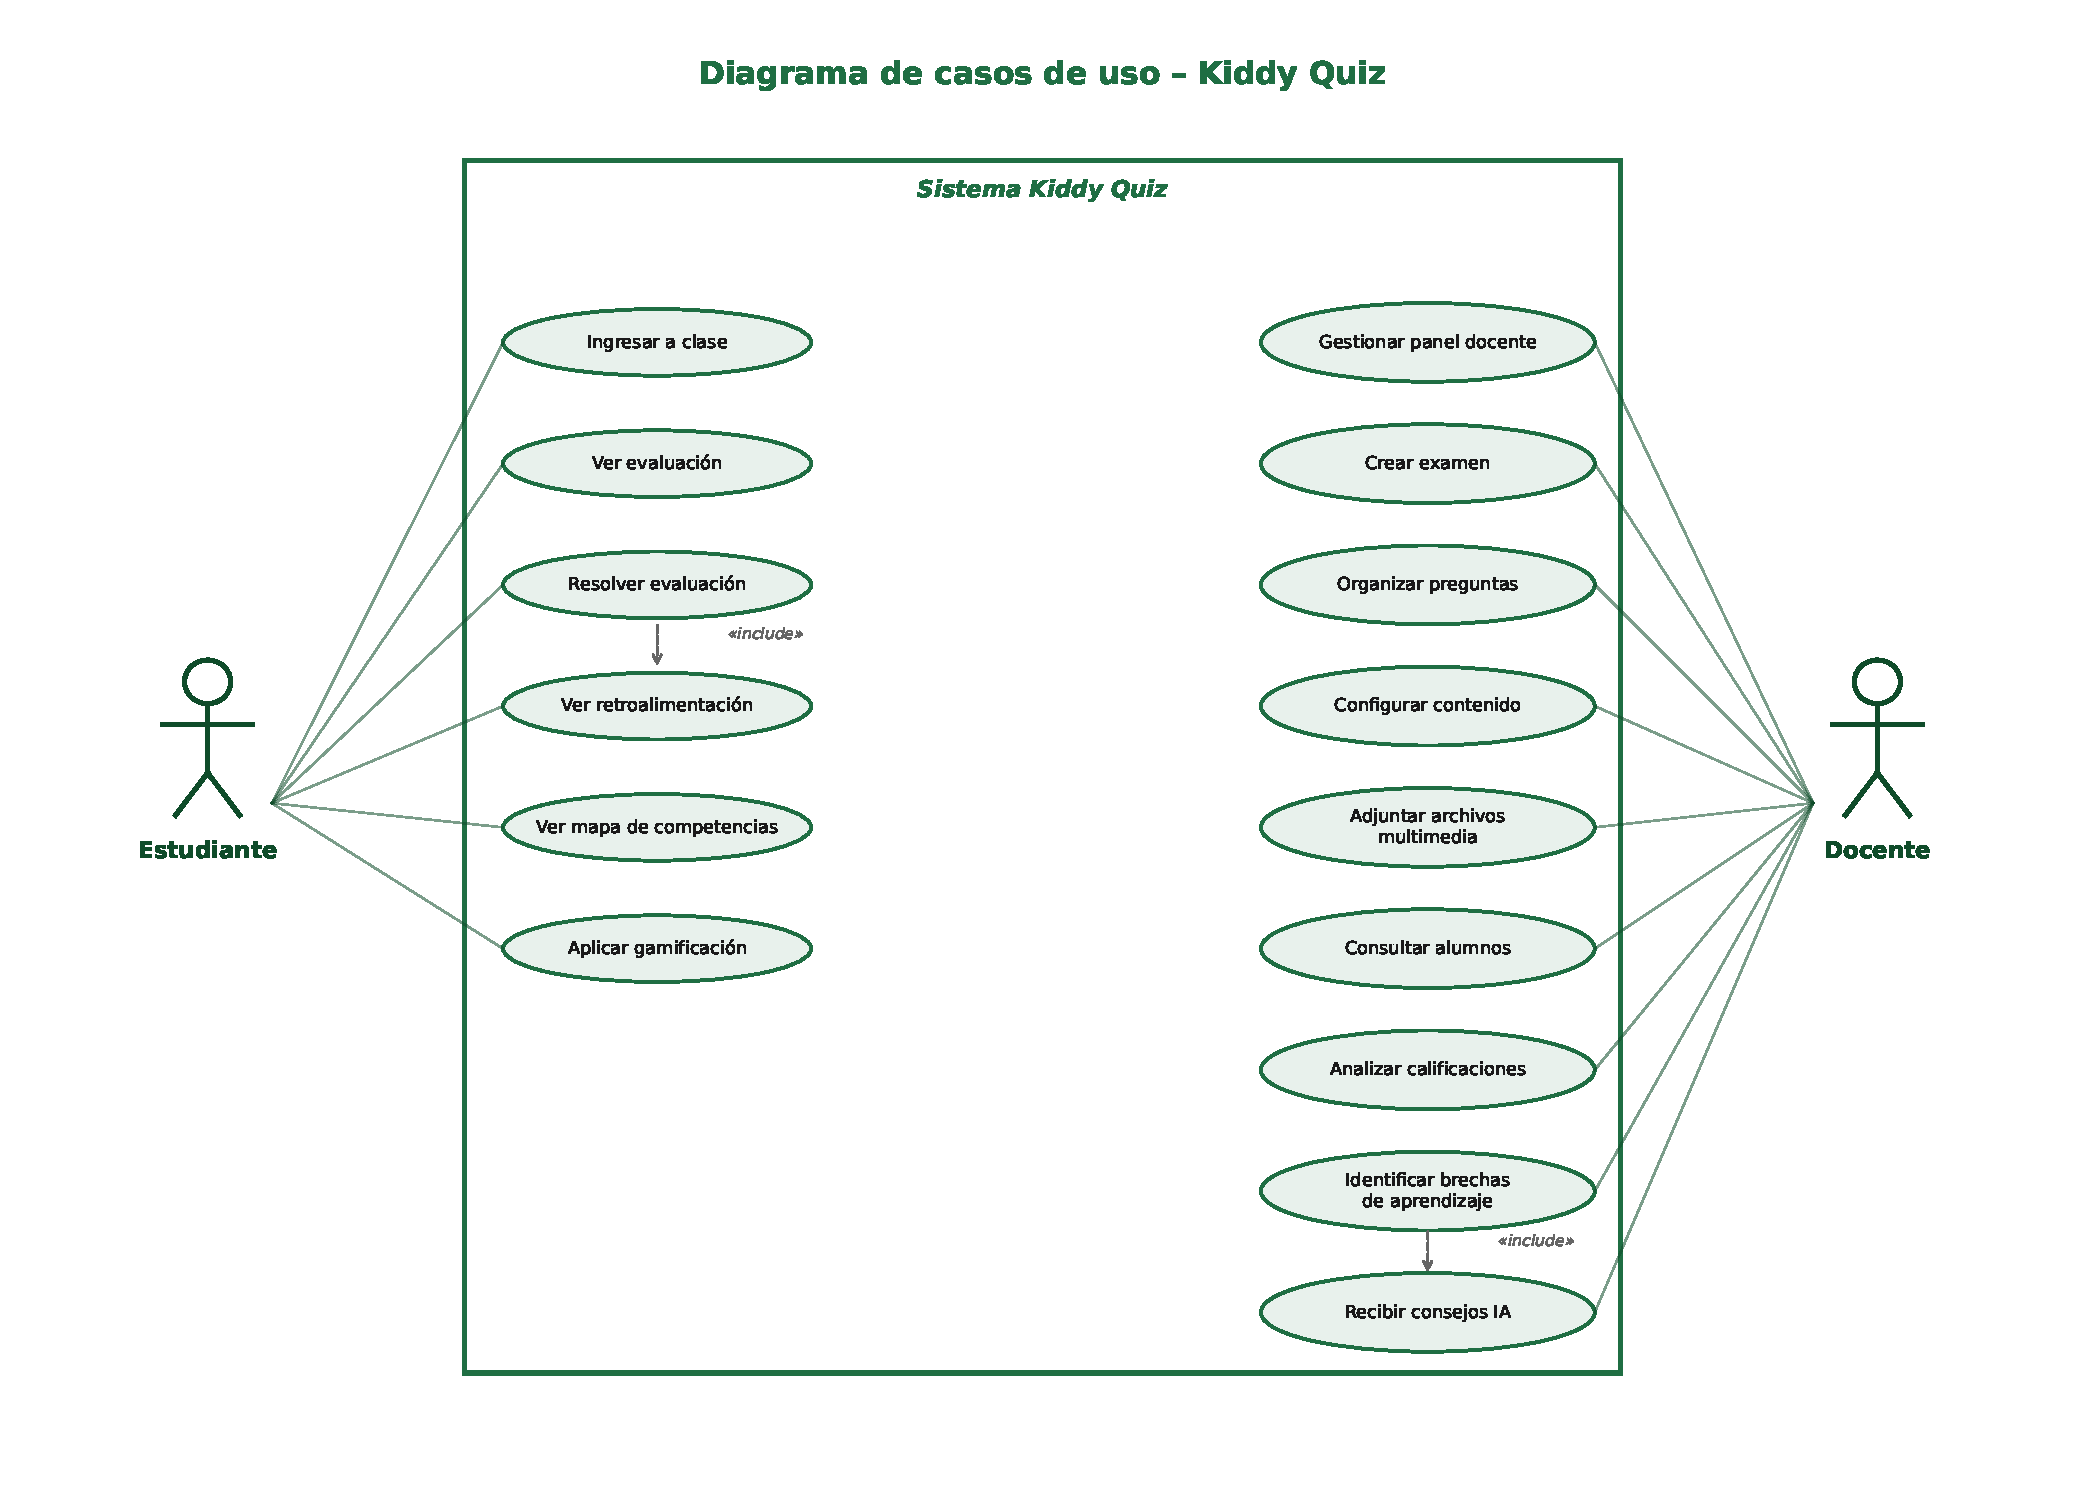
\includegraphics[width=\textwidth]{figuras/fig03_casos_uso.pdf}
\fuenteautor
\end{figure}

\section{Manual de usuario de la aplicación Kiddy Quiz}

A continuación se presenta el resumen del manual de usuario de la aplicación Kiddy Quiz. La versión completa con capturas adicionales se distribuye en formato PDF como complemento del presente documento.

\textbf{Acceso al sistema.} El usuario accede mediante \texttt{https://kiddyquiz.app} introduciendo sus credenciales. Tras autenticarse con éxito, el sistema redirige al panel correspondiente según el rol (estudiante o docente).

\textbf{Perfil del estudiante.} Una vez en el panel, el estudiante puede unirse a una clase mediante un código de acceso provisto por su docente. Las evaluaciones disponibles se muestran como tarjetas visuales con pictogramas. Al seleccionar una evaluación, el estudiante visualiza la primera pregunta acompañada de apoyos visuales y, cuando aplica, una opción de lectura por síntesis de voz. Al terminar, el sistema invoca a Gemini AI para generar un mensaje motivacional personalizado, junto con un desglose por áreas evaluadas (véase la Ilustración~\ref{fig:modulo_retro}).

\textbf{Perfil del docente.} El docente accede a un panel central donde puede crear clases, gestionar la lista de estudiantes y administrar evaluaciones. La creación de un examen sigue tres pasos: (i) configuración general (título, dificultad, duración); (ii) adición de preguntas mediante el editor con \textit{Drag \& Drop}; (iii) publicación o programación temporal. Los reportes consolidan el promedio global, la evolución cronológica del puntaje, las áreas fuertes y débiles y permiten exportar a Excel.

\textbf{Recuperación ante incidentes.} En caso de pérdida de conexión durante una evaluación, el sistema persiste localmente las respuestas registradas y las sincroniza automáticamente al recuperarse la conexión. Si el token JWT expira, el usuario es redirigido al login con un mensaje informativo.
